%!TeX root=../thesis.tex
\tikzset{every picture/.style={line width=0.75pt}} % Set default line width to 0.75pt

\chapter{Implementation}

This section presents the implementation of the algorithm based on the work of \cite{Joos_2020}. For each step, we provide the corresponding pseudocode and demonstrate the correctness of the algorithm.

\section{Definitions, Notations and Conventions}


Throughout this chapter, we use some definitions and conventions to make the code simpler.

The total number of vertices is denoted by $n$, and the collection of 
graphs is represented by $G = \{G_1, G_2, \dots, G_n\}$, where each graph $G_i$ 
satisfies Dirac's condition. $d(c, v)$ is the degree of vertex $v$ in graph $G_c$.
$V(X)$ and $A(X)$ represents the sets of vertices and edges of object $X$, respectively. $N_J(X)$ is the set of neighbors of $X$ on graph $J$.

The pseudocode is written using Python methods and conventions, such as array slicing and 
list appending.

\subsection{Structures and Functions Abstractions}


Let's define some abstract structures and functions.

\subsubsection{Structure of $edge(u, v, c)$}

Each edge in $G$ has three attributes:

\begin{itemize}
    \item $u$, $v$: vertices connected by the edge
    \item $c$: color of the edge, which also indicates that the edge belongs to graph $G_c$
\end{itemize}

\subsubsection{Structure of $Path$}

Each path contains two dynamic arrays:

\begin{itemize}
    \item $vertices$: an array of $vertex$
    \item $edges$: an array of $edge$
\end{itemize}

If the $Path$ is not empty, it is guaranteed that size of 
$vertices$ is equal to size of $edges$ plus one. We 
also added the constraint that a $Path$ can't contain repeated 
vertices or edge colors.

This structure has the following methods:

\begin{itemize}
    \item \texttt{pop\_back()}: removes the last vertex and edge from the path
    \item \texttt{back()}: returns the last vertex of the path
    \item \texttt{size()}: returns the size of the path
\end{itemize}

\subsubsection{Structure of $Cycle$}

Same Structure as $Path$. The only difference is that a cycle contains
at least three vertices and $vertices$ length is equal to $edges$ length.

Also, this structure has only one method, \texttt{size()}, which returns the size of the cycle.

\subsubsection{Function $check\_edge(G, u, v, c)$}

This function takes four parameters:

\begin{itemize}
    \item $G$: the collection of graphs
    \item $u$ and $v$: vertices of the edge
    \item $c$: color of the edge
\end{itemize}

If the edge $\{u, v\}$ belongs to $G_c$, the function returns this edge. Otherwise, it returns $None$. The function operates in constant time $O(1)$ since we can implement it using a three-dimensional matrix, which requires $O(n^3)$ memory.

\section{Flowchart}

The algorithm begins with a single object representing an empty path. At 
each iteration, the algorithm processes this object, which may be either 
a path or a cycle of length $\ell$, and transforms it into a new object. 
The result could be a cycle of length $\ell$, a cycle of length $\ell+1$, or 
a path of length $\ell+1$, as shown in the flowchart below.

\begin{figure}[H]
    \centering
    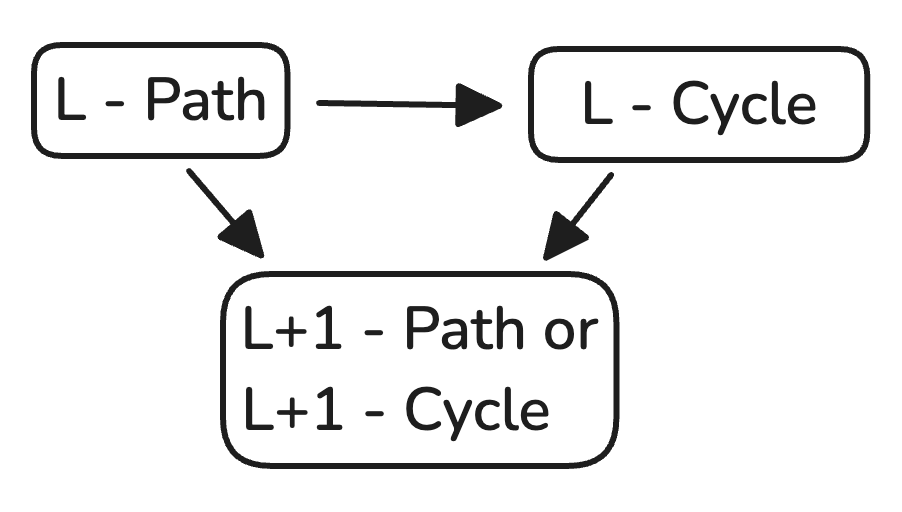
\includegraphics[width=0.3\textwidth]{figuras/flowchart.png}
    \caption{Flowchart of the algorithm}
    \label{fig:flowchart}
\end{figure}

We will assume the algorithm is processing a graph with at
least $6$ vertices. The other cases were already covered by brute force.
The image below shows the possible cases the algorithm can find:

\begin{figure}[H]
    \centering
    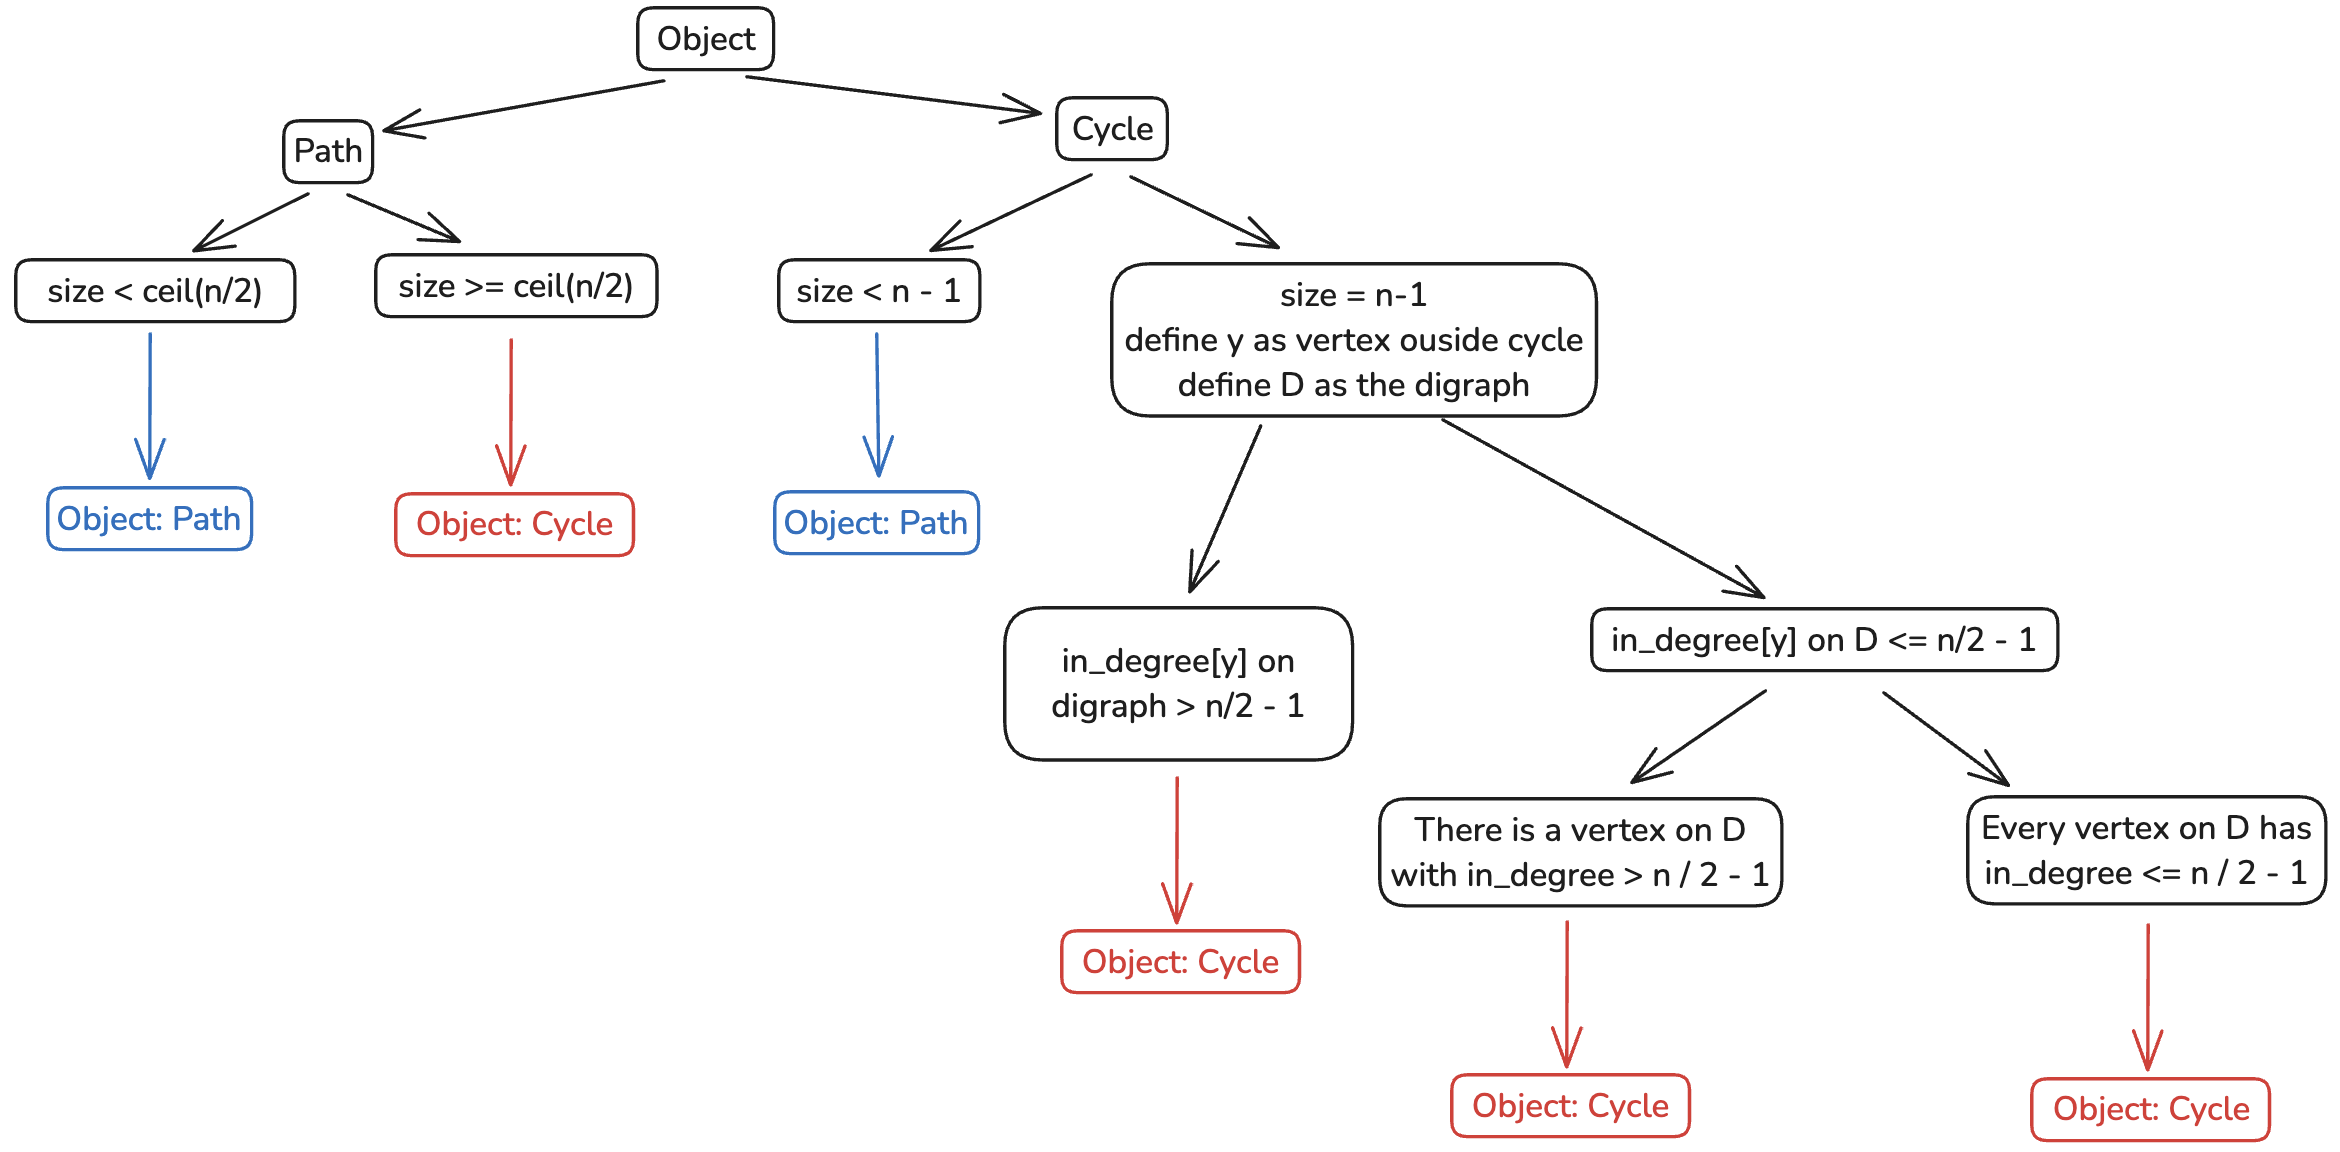
\includegraphics[width=1\textwidth]{figuras/flowchart_case.png}
    \caption{Possible cases the algorithm can find}
    \label{fig:flowchart_cases}
\end{figure}

\subsection{Path of Length \( \ell \)}

In this case, we start with a path \( P = (x_0, e_0, \dots, x_{\ell-1}, e_{\ell-1}, x_{\ell}) \) of length \( \ell \). 
To assist in this process, we define the following variables:

\begin{itemize}
    \item \texttt{colors\_in\_path}: An array of size \( n \) where \texttt{colors\_in\_path[i]} is \texttt{True} if color \( i \) is used in the edges of the path.
    \item \texttt{vertices\_in\_path}: An array of size \( n \) where \texttt{vertices\_in\_path[i]} is \texttt{True} if vertex \( i \) is included in the path.
\end{itemize}

Let's divide the proof into two cases: when \( \ell \geq \left \lceil \frac{n}{2} \right \rceil \) and when \( \ell < \left \lceil \frac{n}{2} \right \rceil \).

\subsubsection{Case 1: \( \ell < \left \lceil \frac{n}{2} \right \rceil \)}

In this case, we select a color \( c \) that is not present among 
the edges of the current path. Since 
\( d(c, x_{\ell}) \geq \left \lceil \frac{n}{2} \right \rceil \), from Dirac's condition, 
and there are at most 
\( \ell < \left \lceil \frac{n}{2} \right \rceil \)
other vertices in the path, there must be a vertex 
\( y \) 
outside the path that is adjacent to 
\( x_{\ell + 1} \) via an edge in \( A(G_c) \). 
This guarantees that we can extend the path to a bigger path.

The code below implements the algorithm:

\begin{algorithm}[H]
    \caption{Path Extension for \( \ell < \left \lceil \frac{n}{2} \right \rceil \)}
    \begin{algorithmic}[1]
        \Function{Extend\_Path\_Small}{$G, P$}
        \State $color\_outside\_path \gets \text{next}(i \text{ for } i \text{ in range(n) if \textbf{not} colors\_in\_path[i]})$

        \For{$i \in [0, \dots, n-1]$}
            \If{\textbf{not} $vertices\_in\_path[i]$}
                \State $edge \gets \text{check\_edge}(G, path.back(), i, color\_outside\_path)$
                \If{$edge \neq \text{None}$}
                    \State \Return Path($G$, $P.vertices + [i]$, $P.edges + [edge]$)
                \EndIf
            \EndIf
        \EndFor

        \State \textbf{assert False, "Should not happen"}
    \EndFunction
    \end{algorithmic}
\end{algorithm}

The time complexity of this function is \( O(n) \). Since we 
only need to find a color that is not in the path’s colors 
,which takes \( O(n) \), and then locate a vertex outside 
the path that connects to the back of the path using the 
function $check\_edge$.

\subsubsection{Case 2: \( \ell \geq \left \lceil \frac{n}{2} \right \rceil \)}

First, remove the last edge and
vertex of the path and let $c_y$ be the color of the removed edge and $c_x$ 
be a color that is not on the path.
We can check if the edge $\{x_0, x_{\ell-1}\}$ belongs to $A(G_{c_x})$ or
to $A(G_{c_y})$. If it does, we just found a cycle of size $l$. 
This can be done with the code below:

\begin{algorithm}[H]
    \caption{Part 1: Path Extension for \( \ell > \left \lceil \frac{n}{2} \right \rceil \)}
    \begin{algorithmic}
        \Function{Extend\_Path\_Big}{$G, P$}
            \State $c_x \gets P.\text{edges}[-1].\text{color}$ \Comment{Color of the last edge in the path}
            \State $c_y \gets \text{next}(i \text{ for } i \text{ in range(n) if \textbf{not} colors\_in\_path[i]})$
            \State $P.\text{pop\_back()}$ \Comment{Remove the last vertex from the path}

            \For{$c \in [c_x, c_y]$}
                \State $edge \gets \text{check\_edge}(G, P.vertices[0], P.vertices[-1], c)$
                \If{$edge \neq \text{None}$}
                    \State \Return Cycle($G$, $P.vertices$, $P.edges + [edge]$) \Comment{Return cycle if found}
                \EndIf
            \EndFor
        \EndFunction
    \end{algorithmic}
\end{algorithm}

The time complexity of this function is $O(n)$, the time needed
to find a color outside the path and create the object Cycle. The other
operations are $O(1)$.

We can now check if there exists a vertex $y$ outside the Path
such that $y$ is connects to the path on vertices $x_0$ and $x_{\ell-1}$
and uses colors $c_x$ and $c_y$, such as in the image below:

\begin{figure}[H]
    \centering
    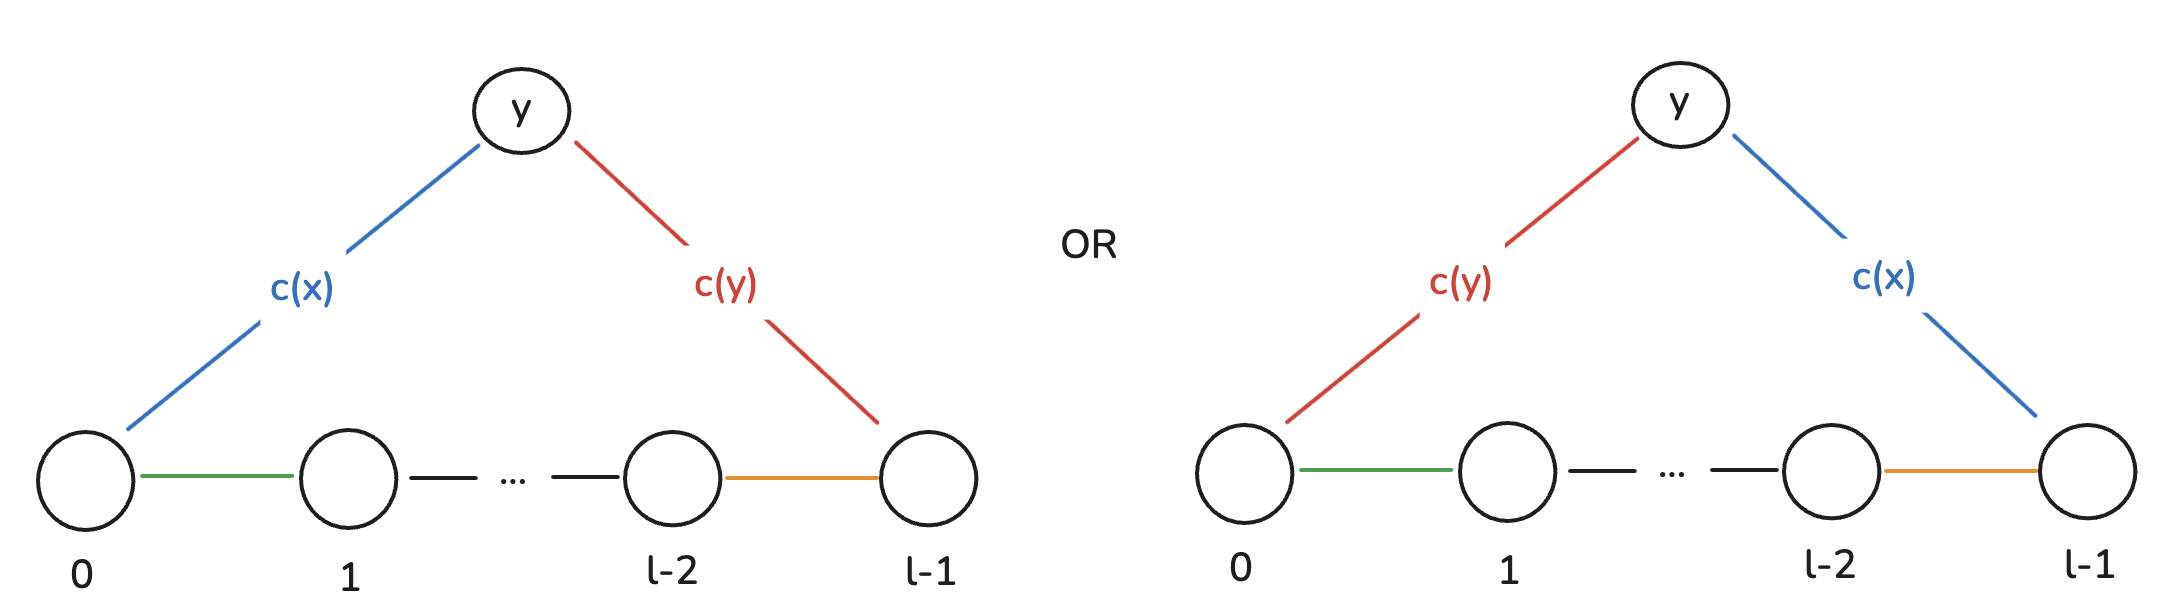
\includegraphics[width=1\textwidth]{figuras/path_vertex_outside.png}
    \caption{Cycle of length \( \ell + 1 \) found}
    \label{fig:path_vertex_outside}
\end{figure}

This part can also be done on $O(n)$ time complexity with
the code below:

\begin{algorithm}[H]
    \caption{Part 3: Path Extension for \( \ell > \left \lceil \frac{n}{2} \right \rceil \)}
    \begin{algorithmic}
        \Function{Extend\_Path\_Big}{$G, P$}
            \For{$[c1, c2] \in [[cx, cy], [cy, cx]]$} \Comment{Try both color pairs}
                \For{$y \in [0, \dots, n-1]$}
                    \If{\textbf{not} $vertices\_in\_path[y]$}
                        \State $edgeX \gets \text{check\_edge}(G, P.vertices[0], y, c1)$
                        \State $edgeY \gets \text{check\_edge}(G, P.vertices[-1], y, c2)$
                        \If{$(edgeX \neq \text{None})$ and $(edgeY \neq \text{None})$}
                            \State \Return Cycle($G$, $P.vertices + [y]$, $P.edges + [edgeY, edgeX]$)
                        \EndIf
                    \EndIf
                \EndFor
            \EndFor

            \State \textbf{assert False, "No valid extension found"}
        \EndFunction
    \end{algorithmic}
\end{algorithm}

Let's define $I_1 = \{i \in [0, \ell - 3]: \{x_0, x_{i + 1}\} \in A(G_{c_x})\}$ and 
$I_2 = \{i \in [1, \ell - 2]: \{x_i, x_{\ell-1}\} \in A(G_{c_y})\}$.

Note that as we did not find a cycle yet, 

$$
|N_{G_{c_x}}(x_0) \backslash V(P)| + |N_{G_{c_y}}(x_\ell) \backslash V(P)| \leq n - \ell,
$$

otherwise, by Pigeonhole Principle, we would have found a cycle
with the previous procedures. Thus, we have that

$$
|I_1| + |I_2| \geq \frac{n}{2} + \frac{n}{2} - |N_{G_cx}(x_1) \backslash V(P)| - |N_{G_cy}(x_\ell) \backslash V(P)| \geq \ell.
$$

As $I_1 \cap I_2 \subseteq [0, \ell - 2]$, from Pigeonhole Principle, $I_1 \cap I_2 \neq \emptyset$. Given an element
$i \in I_1 \cap I_2$, we can build a cycle with size $\ell$ with
the following crossing:

\begin{figure}[H]
    \centering
    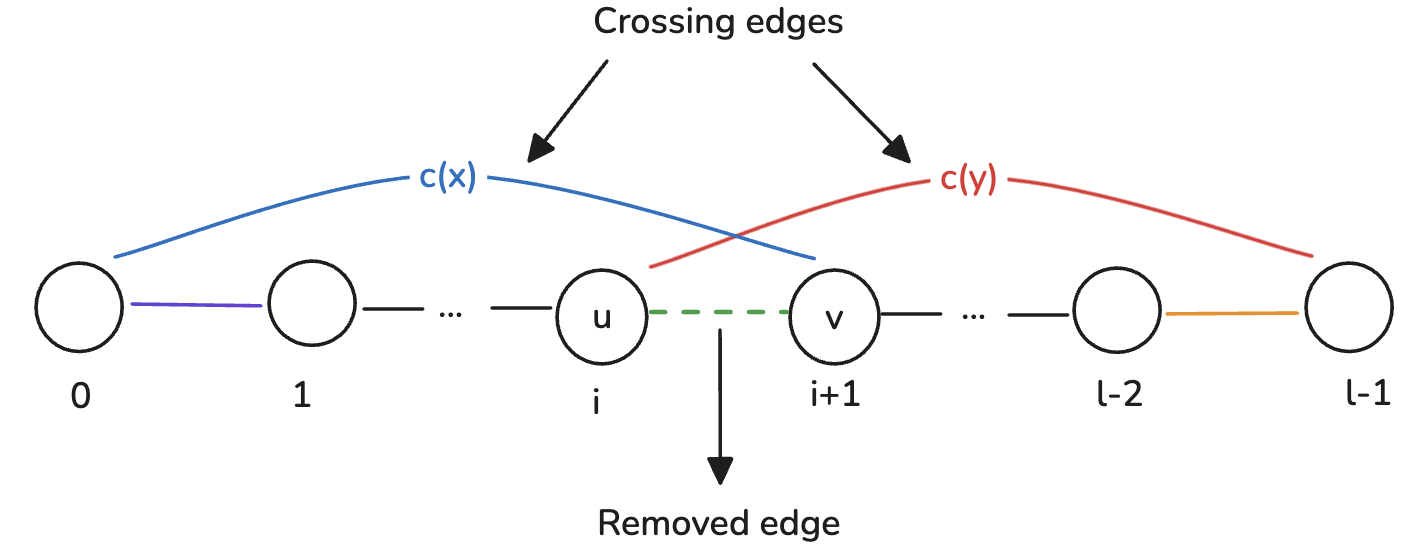
\includegraphics[width=1\textwidth]{figuras/path_cycle_crossing.png}
    \caption{Cycle of length \( \ell + 1 \) found}
    \label{fig:path_cycle_crossing}
\end{figure}

Then, for this case, we just need to find an intersection
for $I_1$ and $I_2$ and build the solution. This can also
be done in $O(n)$ with the code below:

\begin{algorithm}[H]
    \caption{Part 3: Path Extension for \( \ell > \left \lceil \frac{n}{2} \right \rceil \)}
    \begin{algorithmic}[1]
        \Function{Extend\_Path\_Big}{$G, P$}
            \For{$i \in [1, \dots, P.vertices.\text{size()} - 1]$}
                \State $u \gets P.\text{vertices}[i]$
                \State $v \gets P.\text{vertices}[i + 1]$
                \State $edgeX \gets \text{check\_edge}(G, P.\text{vertices}[0], v, cx)$
                \State $edgeY \gets \text{check\_edge}(G, u, P.\text{vertices}[-1], cy)$
                \If{$(edgeX \neq \text{None})$ and $(edgeY \neq \text{None})$} 
                    \State $vertices \gets P.\text{vertices}[:i + 1] + [y] + P.\text{vertices}[i + 1:-1][::-1]$
                    \State $edges \gets P.\text{edges}[:i] + [edgeY] + P.\text{edges}[i + 1:][::-1] + [edgeX]$
                    \State \Return Cycle($G$, $vertices$, $edges$)
                \EndIf
            \EndFor
            \State \Return \text{None} \Comment{Return None if no cycle found}
        \EndFunction
    \end{algorithmic}
\end{algorithm}


\subsection{Cycle of length \( \ell \)}

In this case, we start with a cycle \( C = \{x_0, e_0, \dots, x_{\ell-1}, e_{\ell-1}, x_{\ell} = x_0\} \) of length \( \ell \).
To assist the process, we define the following variables:

\begin{itemize}
    \item \texttt{colors\_in\_cycle}: An array of size \( n \) where \texttt{colors\_in\_cycle[i]} is \texttt{True} if color \( i \) is used in the edges of the cycle.
    \item \texttt{vertices\_in\_cycle}: An array of size \( n \) where \texttt{vertices\_in\_cycle[i]} is \texttt{True} if vertex \( i \) is included in the cycle.
\end{itemize}

These variables can be calculated in \( O(n) \) time complexity. We may assume the cycle is of length at least \( \left \lceil \frac{n}{2} \right \rceil \).
Let's divide the proof into two cases: when \( \ell < n - 1 \) and when \( \ell = n - 1 \).

\subsection{Case 1: \(\left \lceil \frac{n}{2} \right \rceil + 1 \leq \ell \leq n - 1 \)}

Let $c_1$ and $c_2$ be two colors that are not in the cycle. Suppose, WLOG, that 
there is an edge $edge(u, v, c_1) \in A(G)$ not incident to the cycle. Then, because
the adjacency of $u$ is at least $\left \lceil \frac{n}{2} \right \rceil$ and the 
length of the cycle is $\ell \geq \left \lceil \frac{n}{2} \right \rceil + 1$, there is at least
one vertex $w$ on the cycle such that $\{u, w\} \in A(G_{c_2})$.

Thus, we can build a path of length $\ell + 1$ by removing the edge as on the diagram below:

\begin{figure}[H]
    \centering
    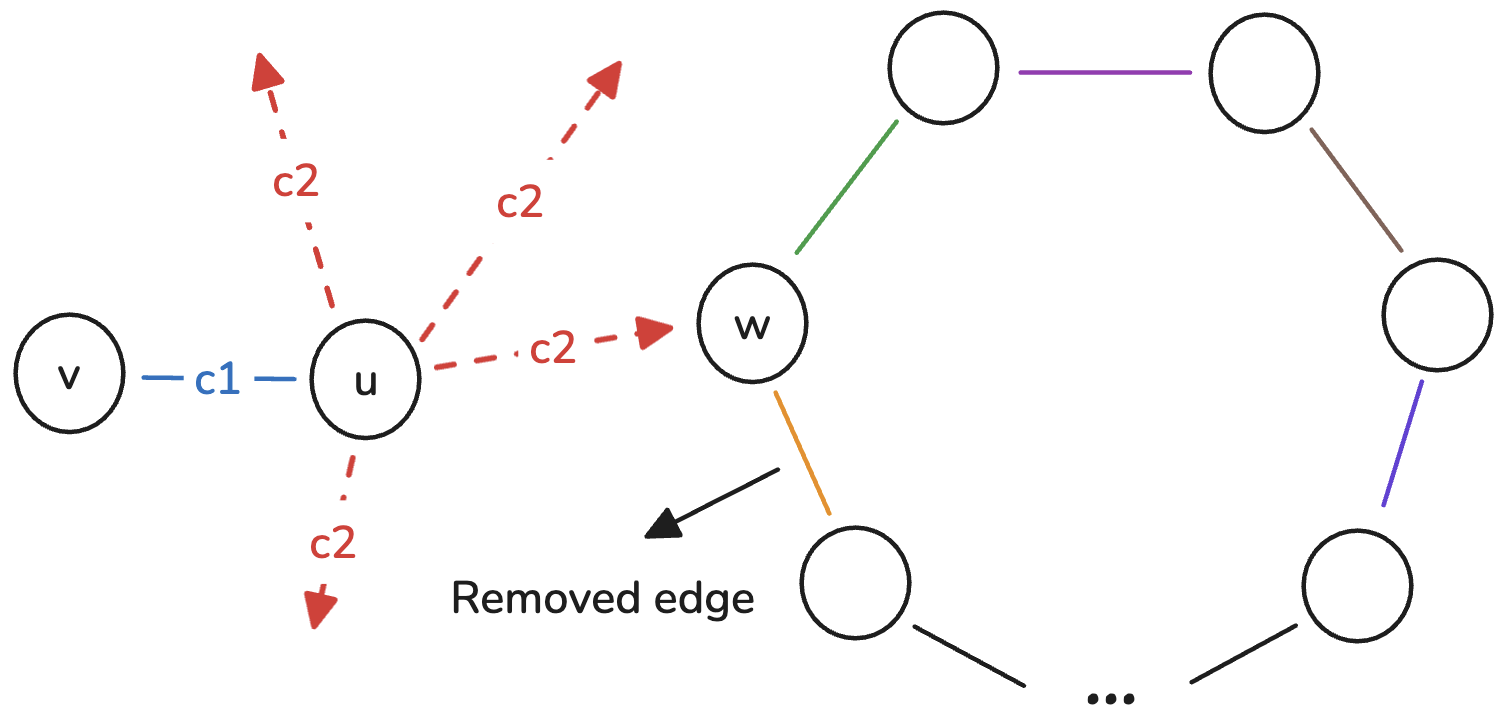
\includegraphics[width=0.7\textwidth]{figuras/cycle_path_extension.png}
    \caption{Path of length \( \ell + 1 \) found}
    \label{fig:cycle_path_extension}
\end{figure}

This can be done in $O(n^2)$ time complexity with the following code:

\begin{algorithm}[H]
    \caption{Part 1: Cycle Extension for \( \ell < n - 1 \)}
    \begin{algorithmic}
        \Function{Extend\_Cycle}{$G, C$}
            \For{$[ci, cj] \in [[c1, c2], [c2, c1]]$} \Comment{Try both color pairs}
                \For{$u \in [0, \dots, n-1]$}
                    \For{$v \in [u + 1, \dots, n-1]$}
                        \If{\textbf{not} $vertices\_in\_cycle[u]$ \text{and} \textbf{not} $vertices\_in\_cycle[v]$}
                            \State $edgeU \gets \text{check\_edge}(G, u, v, ci)$
                            \If{$edgeU \neq \text{None}$}
                                \For{$k \in [0, \dots, C.vertices.\text{size()} - 1]$}
                                    \State $w \gets C.vertices[k]$
                                    \State $edgeW \gets \text{check\_edge}(G, w, u, cj)$
                                    \If{$edgeW \neq \text{None}$}
                                        \State $vertices \gets [u, v] + C.vertices[k:] + C.vertices[:k]$
                                        \State $edges \gets [edgeU, edgeW] + C.edges[k:]$
                                        \State \hspace{3em} $+ C.edges[:k]$
                                        
                                        \State \Return $\text{Path}(G, vertices, edges)$
                                    \EndIf
                                \EndFor
                                \State \textbf{assert False, "Should not reach here"}
                            \EndIf
                        \EndIf
                    \EndFor
                \EndFor
            \EndFor
            \State \textbf{...}
        \EndFunction
    \end{algorithmic}
\end{algorithm}

The complexity is in fact $O(n^2)$ because once we find valid edge $edgeU$, we 
just make a linear search for a valid vertex $w$ in the cycle, that will 
certainly be found.

From now on, for every vertex $u$ outside the cycle, every edge of colors $c_1$ and $c_2$ incident to 
$u$ must also be incident to the cycle. 
Take a vertex $u$ outside the cycle and let

$$
I_1 \coloneqq \{i \in [0, \ell - 1]: \{u, x_{i + 1}\} \in A(G_{c_1})\} \text{ and } I_2 \coloneqq \{i \in [0, \ell - 1]: \{x_i, u\} \in A(G_{c_2})\}.
$$

We have that $|I_1| + |I_2| = |N_{G_{c_1}}(u)| + |N_{G_{c_2}}(u)| > \ell$. Thus, 
from Pigeonhole Principle, $I_1 \cap I_2 \neq \emptyset$. In this case, we can build a cycle of length $\ell + 1$
such as in the image below:

\begin{figure}[H]
    \centering
    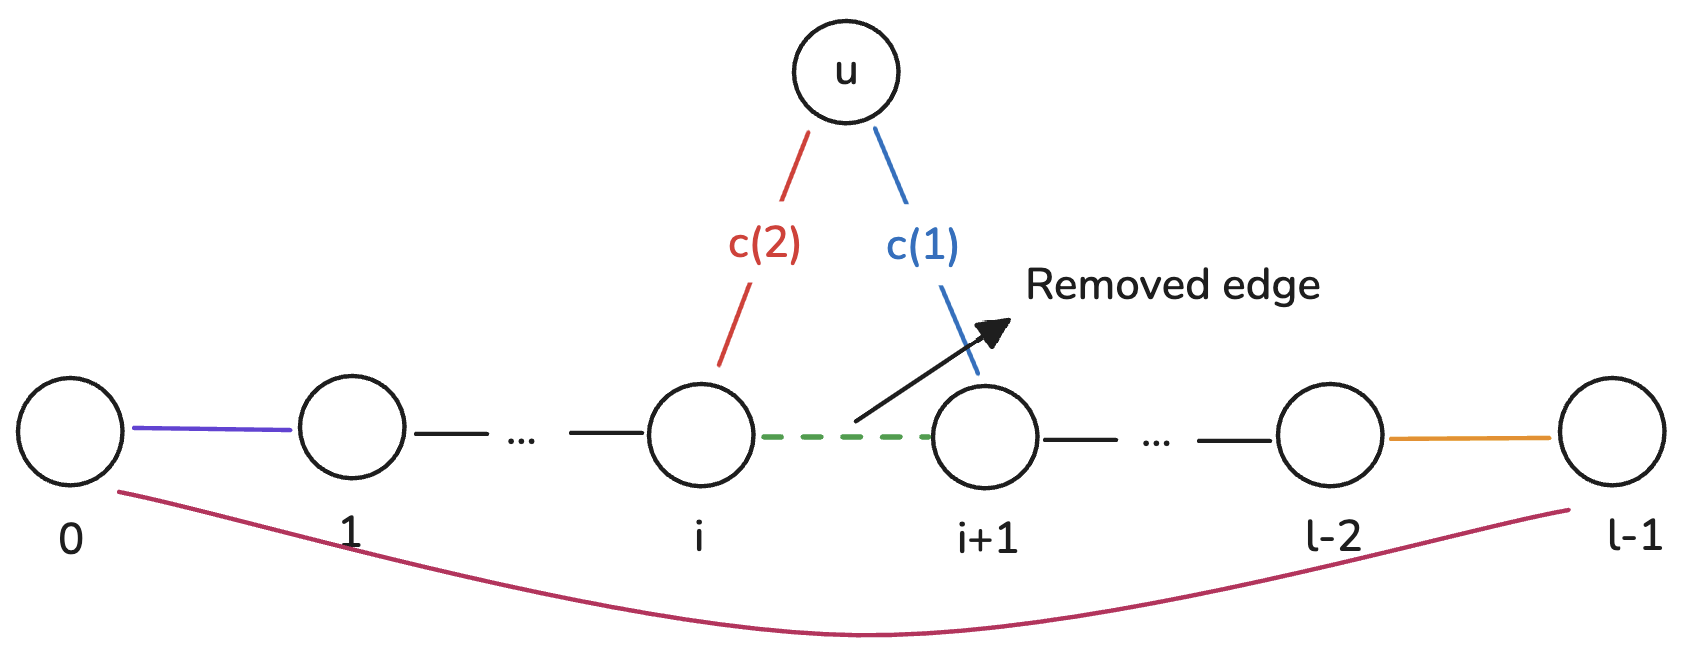
\includegraphics[width=0.7\textwidth]{figuras/cycle_cycle_extension.png}
    \caption{Cycle of length \( \ell + 1 \) found}
    \label{fig:cycle_cycle_extension}
\end{figure}

The code for finding this cycle is shown below:

\begin{algorithm}[H]
    \caption{Part 2: Cycle Extension for \( \ell < n - 1 \)}
    \begin{algorithmic}
        \Function{Extend\_Cycle}{$G, C$}
            \State $u \gets \text{next}(i \text{ for } i \text{ in range(n) if \textbf{not} } colors\_in\_cycle[i])$
            \For{$i \in [0, \dots, C.vertices.\text{size()} - 1]$}
                \State $edge1 \gets \text{check\_edge}(G, u, C.vertices[i + 1], c1)$
                \State $edge2 \gets \text{check\_edge}(G, u, C.vertices[i], c2)$
                
                \If{$edge1 \neq \text{None} \text{ and } edge2 \neq \text{None}$}
                    \State $vertices \gets C.vertices[i + 1:] + C.vertices[:i + 1] + [u]$

                    \State $edges \gets C.edges[i + 1:] +$
                    \State \hspace{3.3em} $C.edges[:i - 1] +$
                    \State \hspace{3.3em} $[edge2, edge1]$
                    \State \Return $\text{Cycle}(G, vertices, edges)$
                \EndIf
            \EndFor
            \State \textbf{assert False, "Should not reach here"}
        \EndFunction
    \end{algorithmic}
\end{algorithm}

This part works in $O(n)$ time complexity, as we as soon as we find a vertex outside the cycle,
we just make a linear search for a crossing and find the solution.

\subsection{Case 2: Cycle of length \( \ell = n - 1 \)}

This is the most complicated case. We are going to define some auxiliary functions
to simplify the code.

\subsubsection{Auxiliary Functions}

\begin{itemize}
    \item \texttt{find\_adjacency(u, color, vertex\_positions)}: This function gives the indexes of the 
    vertices that are adjacent to $u$ with color $color$, based on the current 
    positions of the vertices. This is useful when we need to change the vertex position in the cycle.
    The algorithm is shown below:

    \begin{algorithm}
        \caption{Find Adjacency Index List for a Given Source and Color}
        \begin{algorithmic}[1]
            \Function{Find\_Adjacency}{$u, color, vertex\_positions$}
                \State $ans \gets []$
                \For{$tgt \in G.\text{adjacency}[color][u]$}
                    \State $ans.\text{append}(vertex\_positions[tgt])$
                \EndFor
                \State \Return $ans$ \Comment{Return the list of positions}
            \EndFunction
        \end{algorithmic}
    \end{algorithm}

    It's complexity is $O(n)$, as we just need to iterate over the adjacency list of $u$ with color $color$.

    \item \texttt{find\_answer(G, y, cy, C, i)}: Let $G$ be the graph collection, $C$ a cycle with
    size $n-1$, $y$ be the only vertex outside the cycle, $c_y$ be the only color
    outside the cycle and $i$ the index of the edge $e_i$ to be removed. This function 
    builds a cycle with size $n$ by removing the edge $e_i$ and adding the edges
    $edge(x_{i}, y, e_i.color)$ and $edge(y, x_{i+1}, c_y)$.

    The algorithm is shown below:

    \begin{algorithm}
        \caption{Find Answer for \( \ell = n - 1 \)}
        \begin{algorithmic}[1]
            \Function{Find\_Answer}{$G, y, cy, C, i$}
                \State $vertices \gets C.vertices[i + 1:] + C.vertices[:i + 1] + [y]$
                \State $edges \gets C.edges[i + 1:] + C.edges[:i]$
                \State \hspace{2.5em} $+ [G.\text{get\_edge}(vertices[-1], y, C.edges[i].color), G.\text{get\_edge}(y, C.vertices[0], cy)]$
                \State \Return $\text{Cycle}(G, vertices, edges)$
            \EndFunction
        \end{algorithmic}
    \end{algorithm}

    The complexity is $O(n)$, as we just need to rotate some lists of size $n$ and the other operations are $O(1)$.
\end{itemize}

\subsubsection{Algorithm}

This case is a bit more complicated. It is always the last iteration of the algorithm and will
find the desired cycle.

Let $y$ and $cy$ be the vertex and color that are not in the cycle. We will rearrange the labels
of the colors such that the remaining color has label $n - 1$. Let's also define the following variables:

\begin{itemize}
    \item \texttt{new\_color\_id}: An array of size \( n \) where \texttt{new\_color\_id[i]} is the new label of color \( i \),
    \item \texttt{vertex\_position\_on\_cycle}: An array of size \( n \) where \texttt{vertex\_position\_on\_cycle[i]} is the position of vertex \( i \) in the cycle.
    \item \texttt{color\_in\_position}: An array of size \( n \) where \texttt{color\_in\_position[i]} is the color of the edge that connects the vertices \( i \) and \( i + 1 \) in the cycle.
\end{itemize}

These variables can be calculated in \( O(n) \) time complexity. The algorithm is shown below:

\begin{algorithm}
    \caption{Part 1: Cycle Extension for \( \ell = n - 1 \)}
    \begin{algorithmic}
        \Function{Extend\_Cycle}{$G, C$}
            \State $new\_color\_id \gets [-1] \times n$

            \State $y \gets \text{next}(i \text{ for } i \text{ in range(n) if \textbf{not} } vertices\_in\_cycle[i])$
            \State $cy \gets \text{next}(i \text{ for } i \text{ in range(n) if \textbf{not} } colors\_in\_cycle[i])$
            \State $new\_color\_id[cy] \gets n - 1$
            
            \For{$i \in [0, \dots, C.\text{size()} - 1]$}
                \State $new\_color\_id[color] \gets i$
                \State $color\_in\_position \gets C.edges[i].color$
            \EndFor
            
            \State $vertex\_position\_on\_cycle \gets [-1] \times n$
            \For{$i \in [0, \dots, C.\text{size()} - 1]$}
                \State $vertex\_position\_on\_cycle[C.vertices[i]] \gets i$
            \EndFor
        \EndFunction
    \end{algorithmic}
\end{algorithm}

Let's build the following digraph on the same vertex set of $G$. There is a visual representation
of the digraph below:

$$
A(D) = \bigcup_{i \in \{0,..., n - 2\}} \{\{x_i, z\} : z \neq x_{i + 1}, \{x_i, z\} \in A(G_{C.edges[i].color})\}.
$$

\begin{figure}[H]
    \centering
    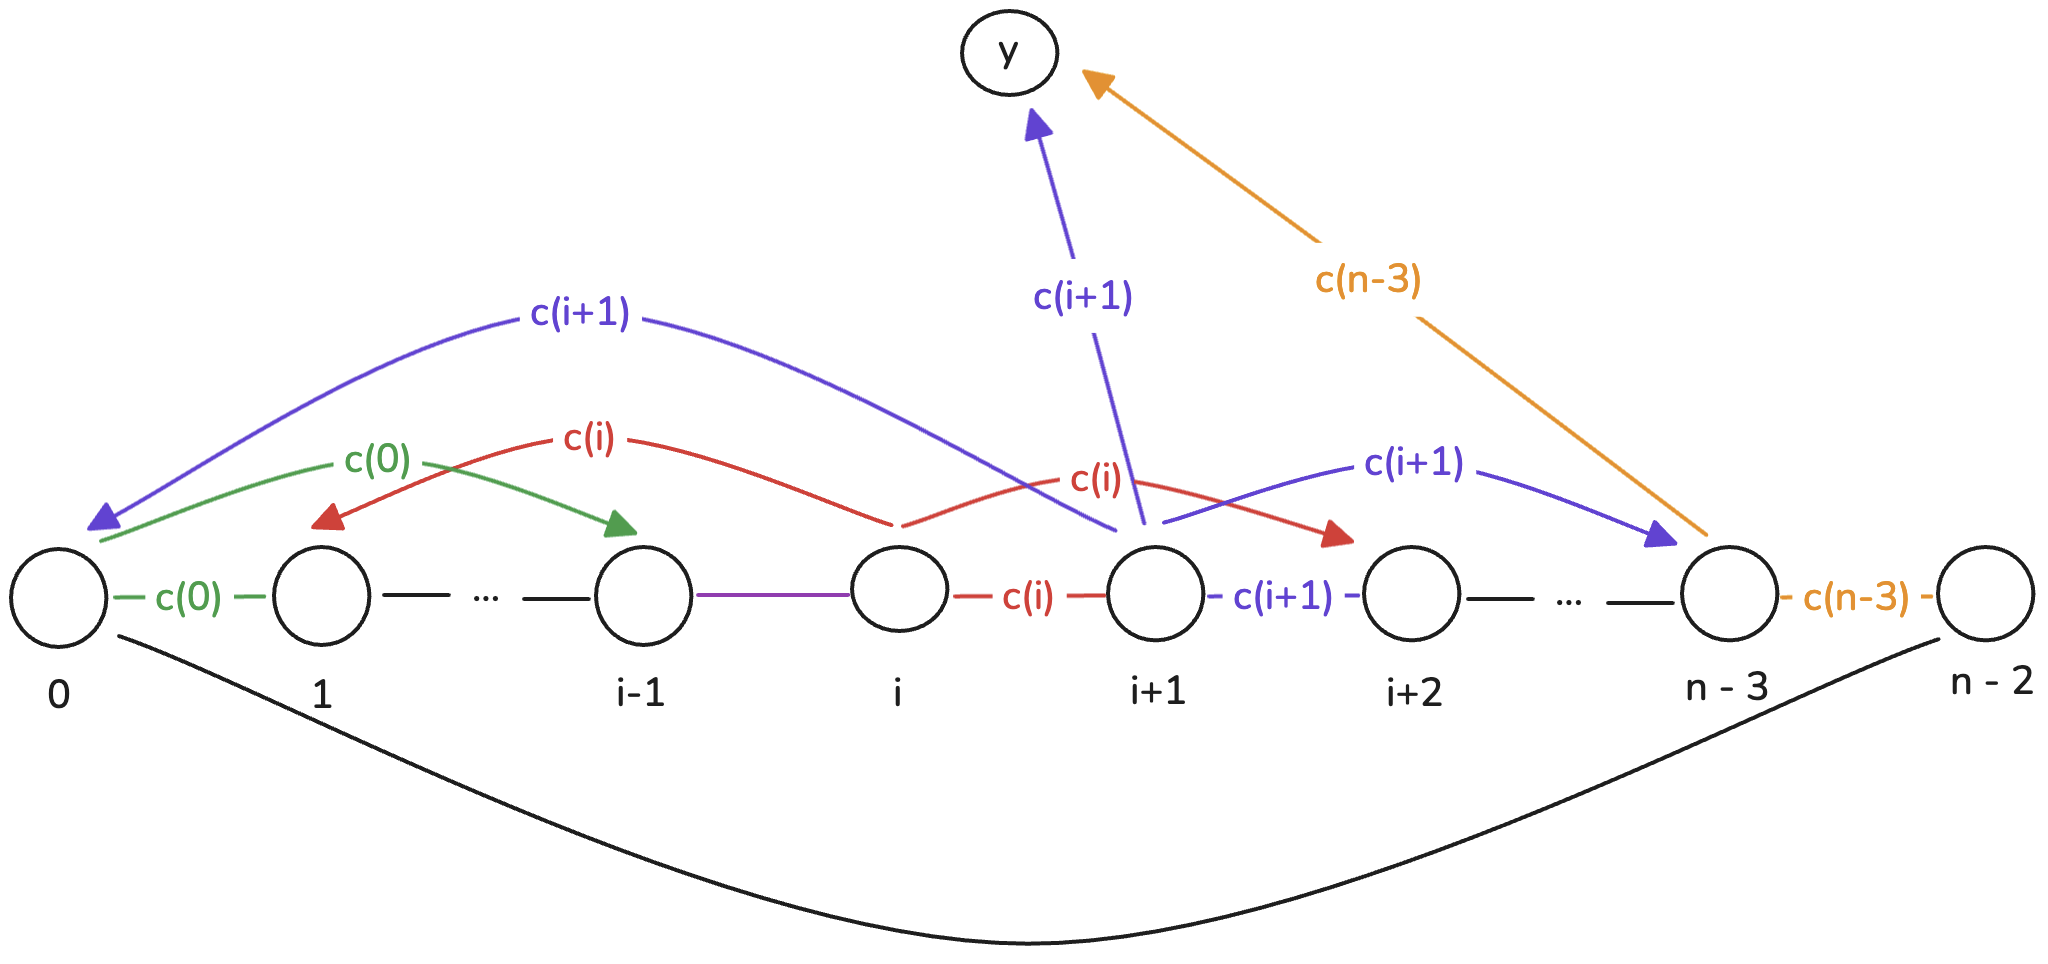
\includegraphics[width=0.7\textwidth]{figuras/cycle_n-1_digraph.png}
    \caption{Digraph construction for the case $l = n - 1$.}
    \label{fig:cycle_n-1_digraph}
\end{figure}

Observe that as $\delta(G_i) \geq \frac{n}{2}$ for all $i \in [0, n - 2]$, thus 
$d^+_{D}(x) \geq \frac{n}{2} - 1$ for every vertex $x$ on the cycle. We get that 
$|A(D)| \geq (n-1)(\frac{n}{2} - 1)$. 

Now, let's define the following variables:

\begin{itemize}
    \item $in\_degree$: An array of size $n$ where $in\_degree[i]$ is the in-degree of vertex $i$ in the digraph $D$.
    \item $incoming\_neighborhood$: An array of size $n$ where $incoming\_neighborhood[i]$ is the list of vertices that have an edge to vertex $i$ in the digraph $D$.
    \item $I \coloneqq \{i \in [n - 1]: \{x_i, y\} \in A(D)\}$
    \item $\bar{I} \coloneqq \{i \in [n - 1]: \{y, x_{i+1}\} \in A(G_{cy})\}$
\end{itemize}

We can build these variables with the following algorithm:

\begin{algorithm}[H]
    \caption{Part 2: Cycle Extension for \( \ell < n - 1 \). Building digraph variables, $I$ and $\bar{I}$}
    \begin{algorithmic}[1]
        \Function{Extend\_Cycle}{$G, C$}
            \State $I \gets []$
            \State $in\_degree \gets [0] \times n$
            \State $incoming\_neighborhood \gets [\text{empty list}] \times n$
            
            \For{$i \gets 0$ to $C.\text{size()} - 1$}
                \State $u \gets C.vertices[i]$
                \State $v \gets C.vertices[(i + 1) \bmod C.\text{size()}]$
                \State $color \gets color\_in\_position[i]$

                \For{$tgt \in G.adjacency[color][u]$}
                    \If{$tgt = v$}
                        \State \textbf{continue}
                    \EndIf
                    
                    \State $in\_degree[tgt] \gets in\_degree[tgt] + 1$
                    \State $incoming\_neighborhood[tgt].append(u)$
                    
                    \If{$tgt = y$}
                        \State $I.append(i)$
                    \EndIf
                \EndFor
            \EndFor
            
            \State $\bar{I} \gets \text{Find\_Adjacency}(y, cy, vertex\_position\_on\_cycle)$
            \State $\bar{I} \gets [(u - 1 + C.\text{size()}) \bmod C.\text{size()} : u \in \bar{I}]$

        \EndFunction
    \end{algorithmic}
\end{algorithm}

The time complexity of this algorithm is $O(n^2)$, as we need to iterate over the vertices of the cycle and iterate over 
it's adjacency list for a specific color. The space complexity is $O(n^2)$, as we need to store the adjacency list of each vertex.

Let's find the answer for the case $d^-_D(y) \geq \frac{n}{2}$. We have that 
$|I| + |\bar{I}|  \geq d^-_D(y) +  \frac{n}{2} $. 
Thus, from Pigeonhole Principle, $I \cap \bar{I} \neq \emptyset$. In this case, we can build 
a cycle of length $n$ with the following crossing, removing the edge $e_i$:

% set scale
\begin{figure}[H]
    \centering
    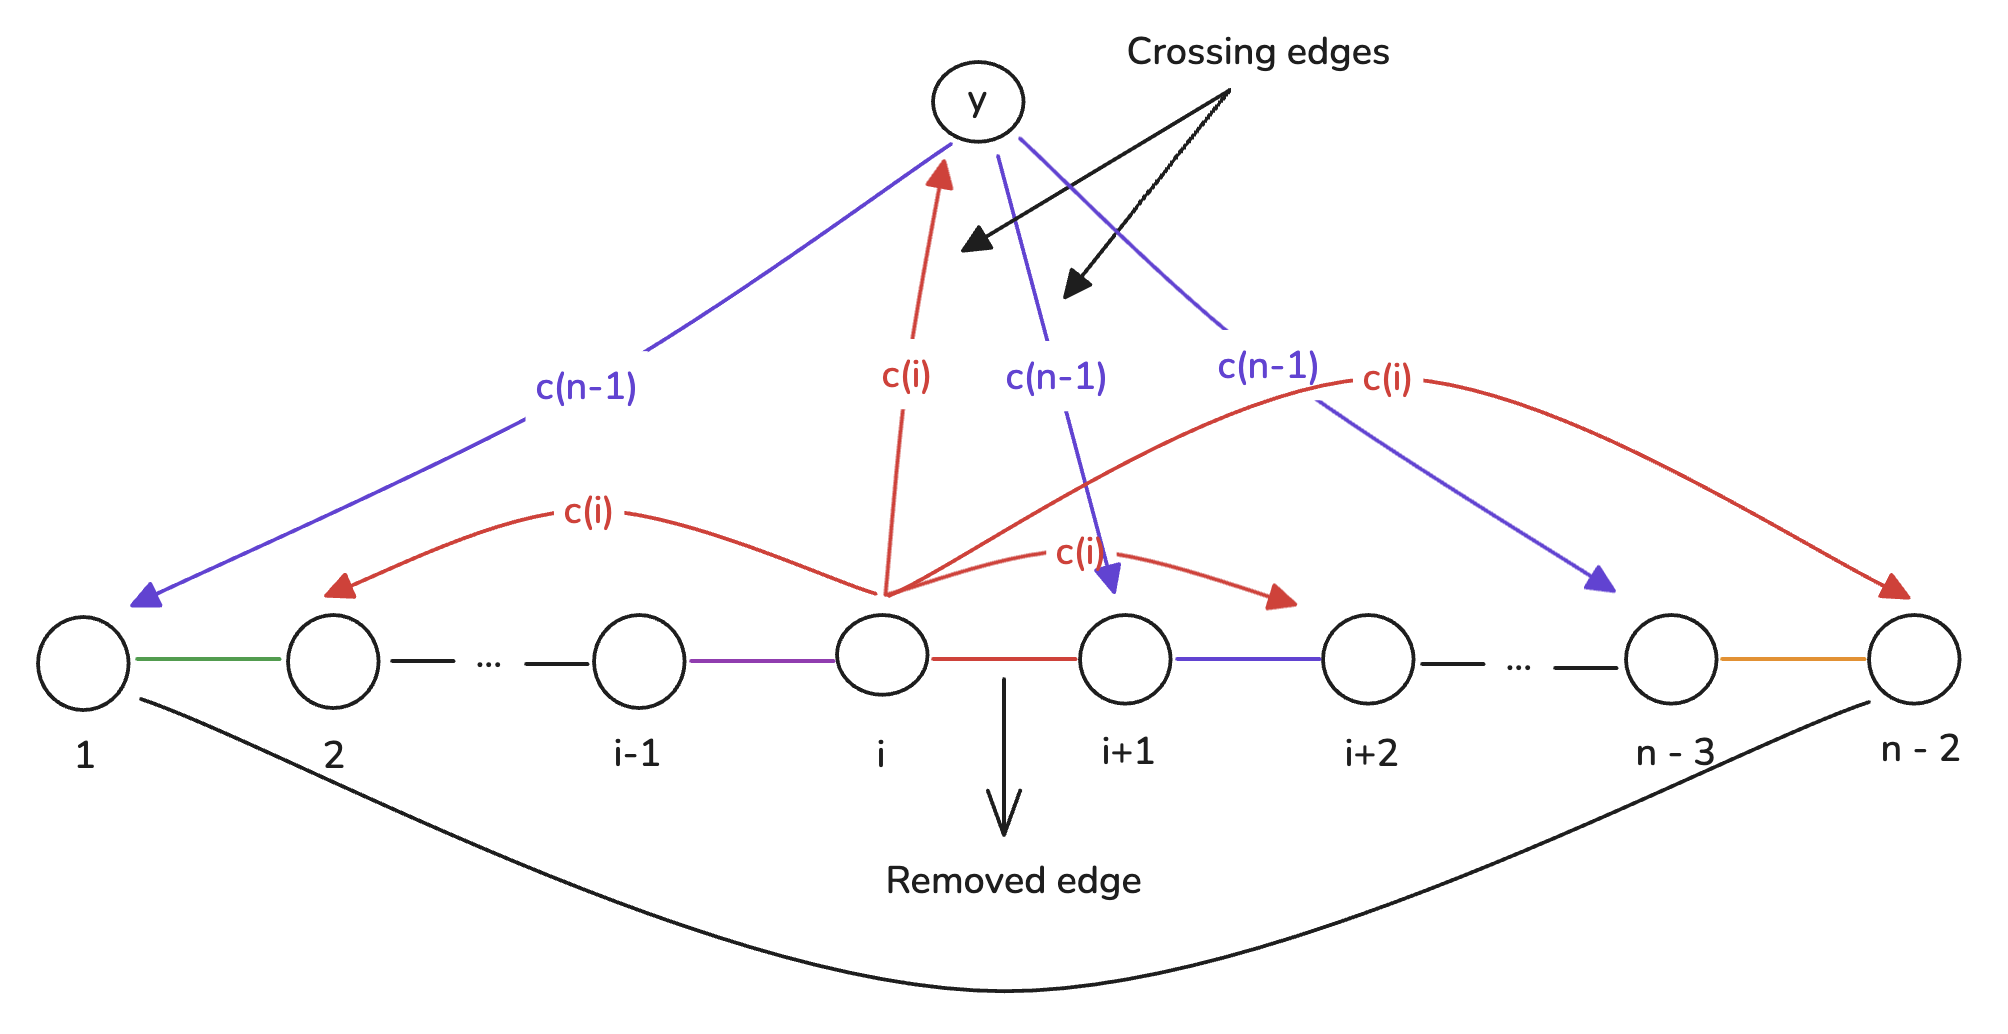
\includegraphics[width=1\textwidth]{figuras/cycle_n-1_crossing_1.png}
    \caption{Crossing for the case $d^-_D(y) \geq \frac{n}{2}$.}
    \label{fig:crossing_case_2}
\end{figure}

To the algorithm part, we can just check the intersection and build the answer.

\begin{algorithm}[H]
    \caption{Part 3: Cycle Extension for \( \ell < n - 1 \). Case \( d^-_D(y) \geq \frac{n}{2} \)}
    \begin{algorithmic}[1]
        \Function{Extend\_Cycle}{$G, C$}
            \For{$i \in I$}
                \If{$i \in \bar{I}$}
                    \State \Return \Call{Find\_Answer}{$G, y, cy, C, i$}
                \EndIf
            \EndFor
        \EndFunction
    \end{algorithmic}
\end{algorithm}

The complexity is $O(n^2)$, as we just need to iterate over $I$, check if it's in $\bar{I}$ and, once we find an element in $\bar{I}$, 
we call the function \texttt{Find\_Answer} that has complexity $O(n)$.

From now on, we will assume that $d^-_D(y) < \frac{n}{2}$. Here we will divide in two cases:

\begin{enumerate}
    \item If there is a vertex $x_i$ such that $d^-_D(x_i) > \frac{n}{2} - 1$.
    \item Otherwise.
\end{enumerate}

Let's start with the first case. We may assume, WLOG, that $d^-_D(x_0) > \frac{n}{2} - 1$.
For considering this, we can just find the vertex with in-degree greater than $\frac{n}{2} - 1$ and rotate the cycle, such as the following algorithm:

\begin{algorithm}[H]
    \caption{Part 4: Cycle Extension for \( \ell < n - 1 \). Case \( d^-_D(y) < \frac{n}{2} \)}
    \begin{algorithmic}[1]
        \Function{Extend\_Cycle}{$G, C$}
            \For{$i \in [0, \dots, C.\text{size()} - 1]$}
                \State $u \gets C.vertices[i]$
                \If{$in\_degree[u] > \frac{n}{2} - 1$}
                    \State $C.vertices \gets C.vertices[i:] + C.vertices[:i]$
                    \State $C.edges \gets C.edges[i:] + C.edges[:i]$
                \EndIf
                % # Rebuild the needed variables
                \For{$j \in [0, \dots, C.\text{size()} - 1]$}
                    \State $color \gets C.edges[j].color$
                    \State $new\_color\_id[color] \gets j$
                    \State $vertex\_position\_on\_cycle[C.vertices[j]] \gets j$
                \EndFor
                \State \textbf{break}
            \EndFor
        \EndFunction
    \end{algorithmic}
\end{algorithm}

The time completity for this is just $O(n)$, as we iterate over the vertices and
as soon as we find the desired vertex, we make $O(n)$ operations to rebuild the needed variables and then we break.

Let's define the following variables:

\begin{itemize}
    \item $I_0 \coloneqq \{i \in [n - 1]: \{x_i, y\} \in A(G_{c_0})\}$
    \item $I_{n-1} \coloneqq \{i \in [n - 1]: \{y, x_{i+1}\} \in A(G_{c_{n-1}})\}$
\end{itemize}

We have that $I_0 + I_{n-1} \geq d(0, y) + d(n-1, y) \geq n$. Thus, 
from Pigeonhole Principle, $I_0 \cap I_{n-1} \neq \emptyset$. Take $j \in I_0 \cap I_{n-1}$.
If $j = 0$, we can just remove the edge $x_0$ and build the cycle of length $n$ 
adding crossing edges $edge(x_0, y, c_0)$ and $edge(y, x_1, c_1)$. So, assume $j \neq 0$.

Let's construct a $G$-transversal path $P$ such as on the figure below:

\begin{figure}[H]
    \centering
    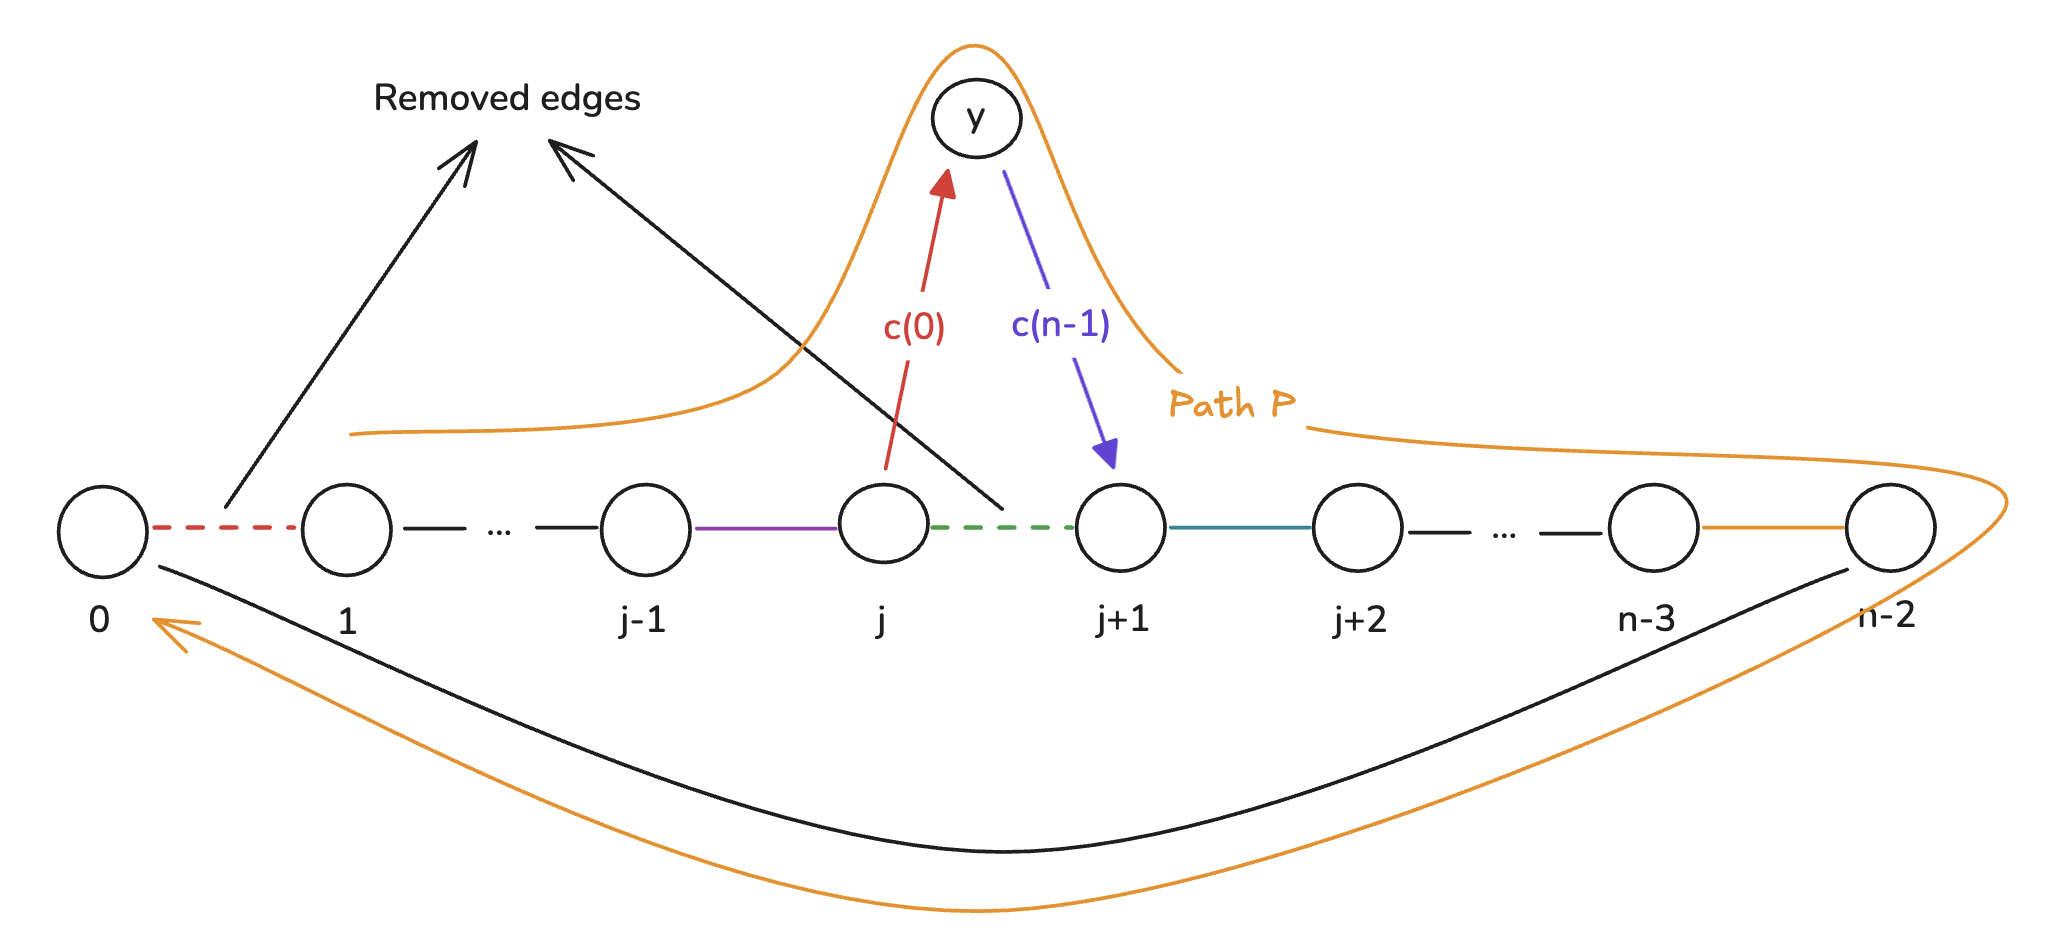
\includegraphics[width=1\textwidth]{figuras/cycle_n-1_build_path.png}
    \caption{Building the transversal path $P$.}
    \label{fig:cycle_n-1_build_path}
\end{figure}

We are going to create the following variables to manipulate the path $P$:

\begin{itemize}
    \item $removed\_color$: The color of the edge outside the path $P$, $C.edges[j].color$;
    \item $P\_vertices$: The vertices of the path $P$, $(x_1, x_2, \dots, x_{j}, y, x_{j+1}, \dots, x_{n-2}, x_{0})$;
    \item $P\_edges$: The edges of the path $P$, $(e_1, e_2, \dots, edge(x_j, y, e_0.color), edge(y, x_{j+1}, cy), \dots, e_{n-2}, e_{0})$;
    \item $P\_pos$: An array to store the new index of each vertex on the path.
\end{itemize}

To compute these variables, we can use the following algorithm:
\begin{algorithm}[H]
    \caption{Part 5: Cycle Extension for \( \ell < n - 1 \). Case \( d^-_D(y) < \frac{n}{2} \)}
    \begin{algorithmic}[1]
        \Function{Extend\_Cycle}{$G, C$}
            \State $j \gets -1$
            \State $removed\_color \gets -1$
            \State $P\_vertices \gets []$
            \State $P\_edges \gets []$
            \State $P\_pos \gets [0] \times n$

            \For{$i \in I_0$}
                \If{$i \in I_{n-1}$}
                    \If{$i = 0$}
                        \State \Return \Call{Find\_Answer}{$G, y, cy, C, i$}
                    \EndIf

                    \State $j \gets i$

                    \State $removed\_color \gets C.edges[j].color$
                    \State $P\_vertices \gets C.vertices[1:j+1] +$
                    \State $\hspace{4.3em} \gets [y] +$
                    \State $\hspace{4.3em} \gets C.vertices[j+1:n] +$
                    \State $\hspace{4.3em} \gets [C.vertices[0]]$

                    \State $P\_edges \gets C.edges[1:j] +$
                    \State $\hspace{4.1em} \gets [get\_edge(G, C.vertices[j], y, C.edges[0].color)] +$
                    \State $\hspace{4.1em} \gets [get\_edge(G, y, C.vertices[(j + 1) \bmod n], cy)] +$
                    \State $\hspace{4.1em} \gets C.edges[j+1:n]$

                    \For{$j \in [0, \dots, n-1]$}
                        \State $P\_pos[P\_vertices[j]] \gets j$
                    \EndFor

                    \State \textbf{break}
                \EndIf
            \EndFor
        \EndFunction
    \end{algorithmic}
\end{algorithm}

The time complexity is $O(n^2)$, as we iterate over $I_0$, check if it's in $I_{n-1}$ and, if it is, we build the path $P$ just once.
To build the path it is just $O(n)$ operations.

Let's now create the following variables:

\begin{itemize}
    \item $J_0 \coloneqq \{i \in [n-2]: edge(P\_vertices[0], P\_vertices[i + 1], removed\_color) \in E(G)\}$
    \item $J_{n-1} \coloneqq \{i \in [n-2]: P\_vertices[i] \in incoming\_neighborhood[P\_vertices[n - 1]]\}$
\end{itemize}


If $edge(P\_vertices[0], P\_vertices[-1], removed\_color)$ in $G$, we can just 
close the cycle adding this edge. Let's assume then we don't have this edge. 
Thus, $|J_0| \geq \delta(G_{removed\_color}) \geq \frac{n}{2}$. Also, as $P\_vertices[-2] \in \{x_{n-2}, y\}$, 
from the construction of $D$ we guarantee that $P\_vertices[n-2] \notin N^-_D(x_0)$
and consequently $|J_{n-1}| \geq \frac{n}{2} - \frac{1}{2}$.

From Pigeonhole Principle, as $|J_0| + |J_{n-1}| \geq n$, we have that $|J_0 \cap J_{n-1}| \geq 2$. Thus,
there is at least one element on $J_0 \cap J_{n-1}$, let's call it $k$, such that $P\_vertices[k] \neq y$.
We can then build the following $G$-transversal cycle:

\begin{figure}[H]
    \centering
    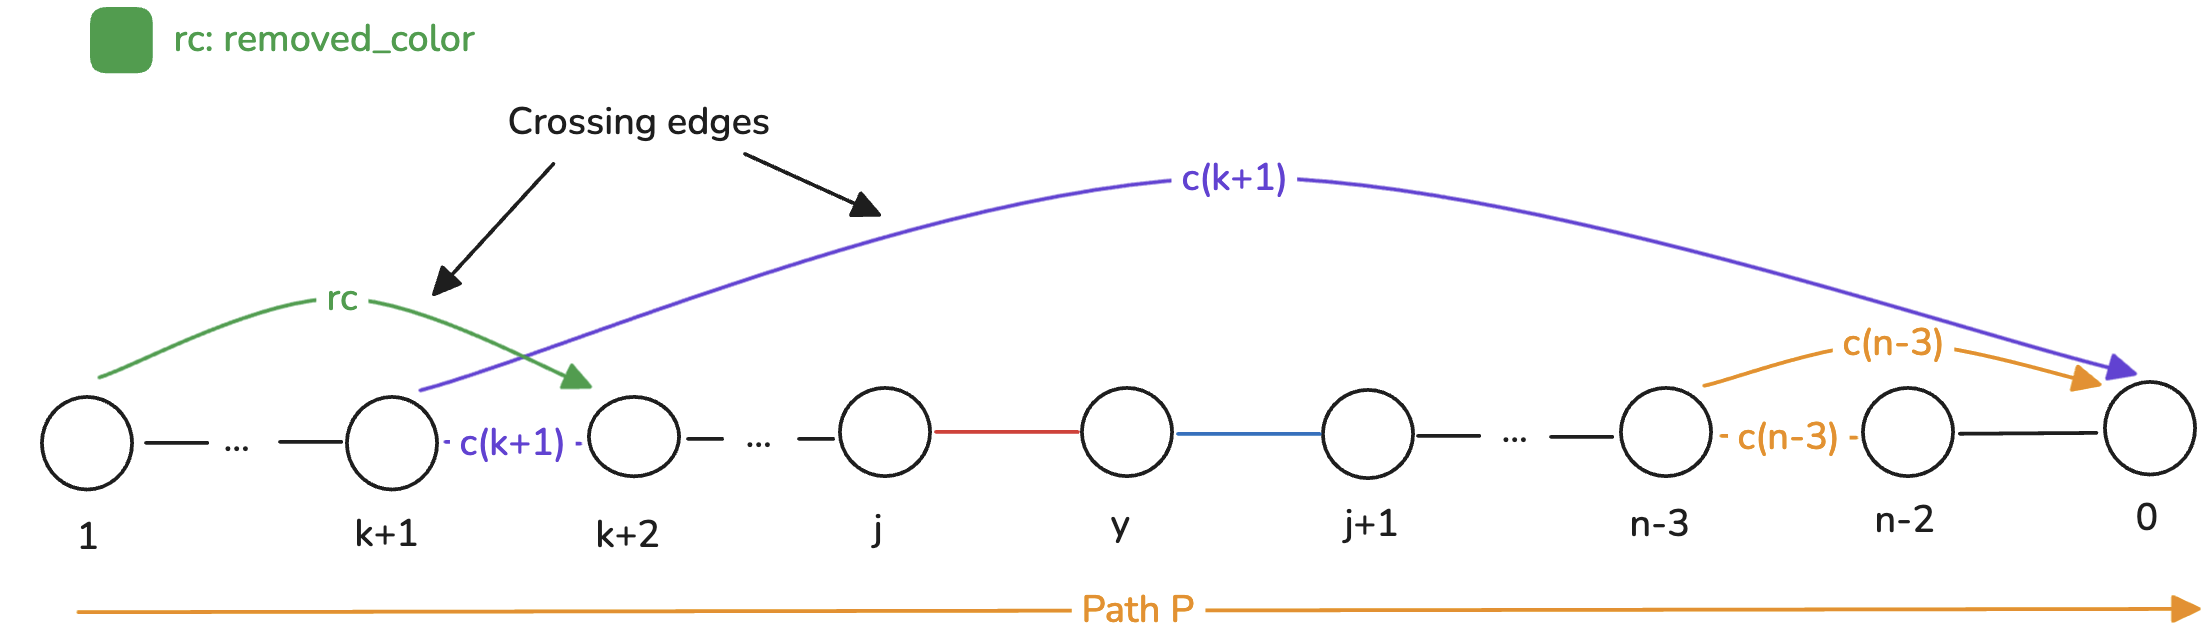
\includegraphics[width=1\textwidth]{figuras/cycle_n-1_cruzamento_not_y.png}
    \caption{Crossing for the case $d^-_D(y) < \frac{n}{2}$ and $P\_vertices[k] \neq y$.}
    \label{fig:cycle_n-1_cruzamento_not_y}
\end{figure}

The algorithm to find the answer in this case is the following:

\begin{algorithm}[H]
    \caption{Part 6: Cycle Extension for \( \ell < n - 1 \). Case \( d^-_D(y) < \frac{n}{2} \)}
    \begin{algorithmic}[1]
        \Function{Extend\_Cycle}{$G, C$}
            \State $edge \gets G.check\_edge(P\_vertices[0], P\_vertices[-1], removed\_color)$
            \If{$edge$ is not $None$}
                \State \Return \Call{Cycle}{$G, P\_vertices, P\_edges + [edge]$}
            \EndIf

            \State $J1 \gets \Call{Find\_Adjacency}{$P\_vertices[0], removed\_color, P\_pos$}$
            \State $J1 \gets [(u - 1 + n) \bmod n : u \in J1]$

            \State $Jn \gets incoming\_neighborhood[P\_vertices[-1]]$
            \State $Jn \gets [P\_pos[u] : u \in Jn]$

            \For{$i \in J1$}
                \If{$i \in Jn$}
                    \If{$P\_vertices[i + 1] = y$}
                        \State \textbf{continue}
                    \EndIf

                    \State $final\_vertices \gets P\_vertices[:i+1] + P\_vertices[i+1:][::-1]$
                    \State $final\_edges \gets P\_edges[:i] +$
                    \State $\hspace{6.7em} [G.get\_edge(P\_vertices[i], P\_vertices[-1], P\_edges[i].color)] +$
                    \State $\hspace{6.7em} P\_edges[i+1:][::-1] +$
                    \State $\hspace{6.7em} [G.get\_edge(P\_vertices[i+1], P\_vertices[0], removed\_color)]$

                    \State \Return \Call{Cycle}{$G, final\_vertices, final\_edges$}
                \EndIf
            \EndFor
        \EndFunction
    \end{algorithmic}
\end{algorithm}

The time complexity is $O(n^2)$, as we iterate over $J_0$ and check 
if the element is in $J_{n-1}$. If it is, we build the cycle and return it, in $O(n)$ operations.
Therefore, for the there exists $x_i$ such that $d^-_D(x_i) > \frac{n}{2} - 1$, we have a total 
complexity of $O(n^2)$.

Now, let's analyze the case where every $x_i$ satisfies $d^-_D(x_i) \leq \frac{n}{2} - 1$.
Define

\begin{equation}
    \mathcal{J} \coloneqq \{i \in [n-1]: d^-_D(x_i) = \lfloor \frac{n}{2} - 1 \rfloor\}.
    \label{eq:J_definition}
\end{equation}

From the construction of $D$, as $d^+_D(y) = 0$ and $d^-_D(y) \leq \frac{n}{2} - 1$, we have:

\begin{equation}
    |A(D - y)| \geq (n - 1) (\frac{n}{2} - 1) - \frac{n}{2} + 1 > (n - 1) (\frac{n}{2} - \frac{3}{2}).
    \label{eq:A_D_minus_y}
\end{equation}

Therefore, from \ref{eq:A_D_minus_y} and \ref{eq:J_definition}, if we analyze
the sum of the in-degrees of the vertices:

\begin{equation}
    |\mathcal{J}| \lfloor \frac{n}{2} - 1 \rfloor + (n - 1 - |\mathcal{J}|) \lfloor \frac{n}{2} - 2 \rfloor \geq |A(D - y)| > (n - 1) \frac{n}{2} - \frac{3}{2}.
\end{equation}

Therefore, $|\mathcal{J}| \geq \frac{n}{2} > \frac{n - 1}{2}$. Defining 
$\mathcal{J}' \coloneqq \{i \in [n - 1]: edge(x_{i+1}, y, c_y) \in A(G)\}$, we have that 
$|\mathcal{J}'| + |\mathcal{J}| \geq n$. From Pigeonhole Principle, there exists 
$j \in \mathcal{J}' \cap \mathcal{J}$. Let's build the following transversal path $Q$:

\begin{figure}[H]
    \centering
    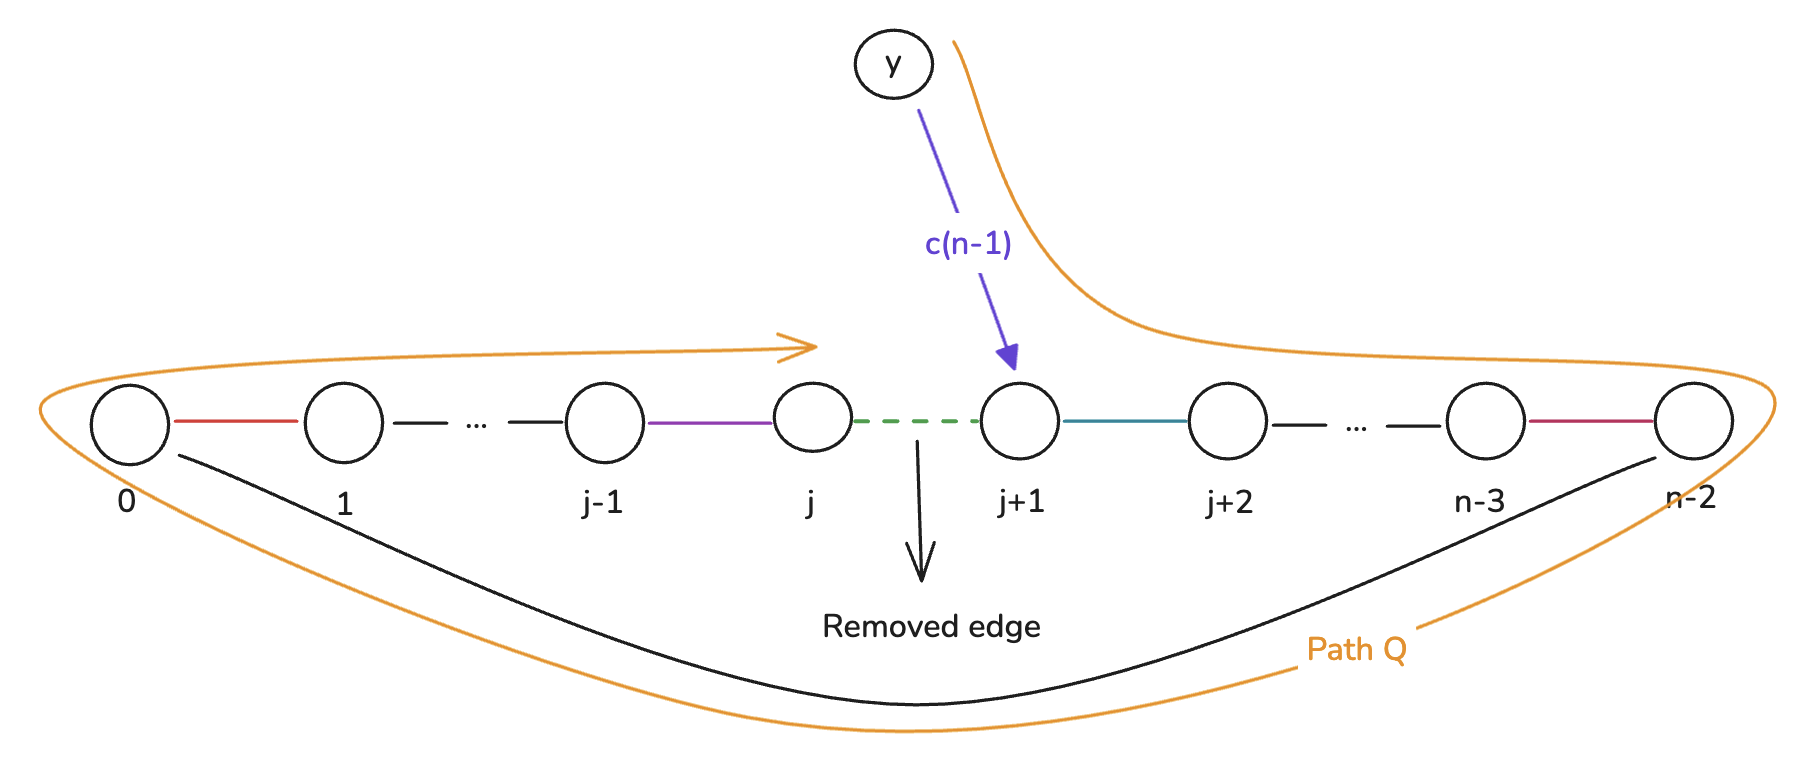
\includegraphics[width=1\textwidth]{figuras/cycle_n-1_path_q.png}
    \caption{Building the transversal path $Q$.}
    \label{fig:cycle_n-1_path_q}
\end{figure}

The algorithm to build $Q$ and get the new missing color is the following:

\begin{algorithm}[H]
    \caption{Part 7: Cycle Extension for \( \ell < n - 1 \). Case \( d^-_D(y) < \frac{n}{2} \)}
    \begin{algorithmic}[1]
        \Function{Extend\_Cycle}{$G, C$}
            \State $Q \gets Path()$
            \State $Q\_pos \gets [0] \times n$
            \State $removed\_color \gets -1$
            \For{$j \in [0, \dots, n - 1]$}
                \State $edge \gets G.get\_edge(y, C.vertices[j], cy)$
                \If{$edge$ is $None$ or $in\_degree[C.vertices[j]] \neq \lfloor \frac{n}{2} - 1 \rfloor$}
                    \State \textbf{continue}
                \EndIf
                \State $Q\_vertices \gets [y] + C.vertices[j + 1:] + C.vertices[:j + 1]$
                \State $Q\_edges \gets [edge] + C.edges[j + 1:] + C.edges[:j]$
                \State $removed\_color \gets C.edges[j].color$
                \For{$i \in [0, \dots, n - 1]$}
                    \State $Q\_pos[Q\_vertices[i]] \gets i$
                \EndFor
                \State $Q \gets$ \Call{Path}{$G, Q\_vertices, Q\_edges$}
                \State \textbf{break}
            \EndFor
        \EndFunction
    \end{algorithmic}
\end{algorithm}

This is $O(n)$ as the most expensive operations are the manipulations on $C$.
Now, define:

\begin{equation}
    J_0 \coloneqq \{i \in [0, n - 3]: \{y, Q.vertices[i+1]\} \in A(G_{removed\_color})\},
\end{equation}
\begin{equation}
    J_{n-1} \coloneqq \{i \in [1, n - 3] : Q.vertices[i] \in incoming\_neighborhood[Q.vertices[n-1]]\}.
\end{equation}

If $\{y, Q.vertices[0]\} \in A(G_{removed\_color})$, we can just close the cycle adding this edge.
Let's assume that this edge is not in $G$. We have that $|J_0| \geq \delta(G_{removed\_color}) \geq \frac{n}{2}$.
Observe that $Q.vertices[0] = y \notin N^-_D(Q_vertices[n - 1])$ and $Q.vertices[n - 2] = C.vertices[j - 1] \notin N^-_D(Q.vertices[n - 1])$,
by the construction of $D$. As $C.vertices[j] \in \mathcal{J}$, we get that
$|J_{n-1}| = \lfloor \frac{n}{2} - 1 \rfloor$. We obtain that $|J_0| + |J_{n-1}| \geq n - 1$.
Thus, from Pigeonhole Principle, there exists $k \in (J_0 \backslash \{0\}) \cap J_{n-1}$. 
We can finally build the following transversal cycle:

\begin{figure}[H]
    \centering
    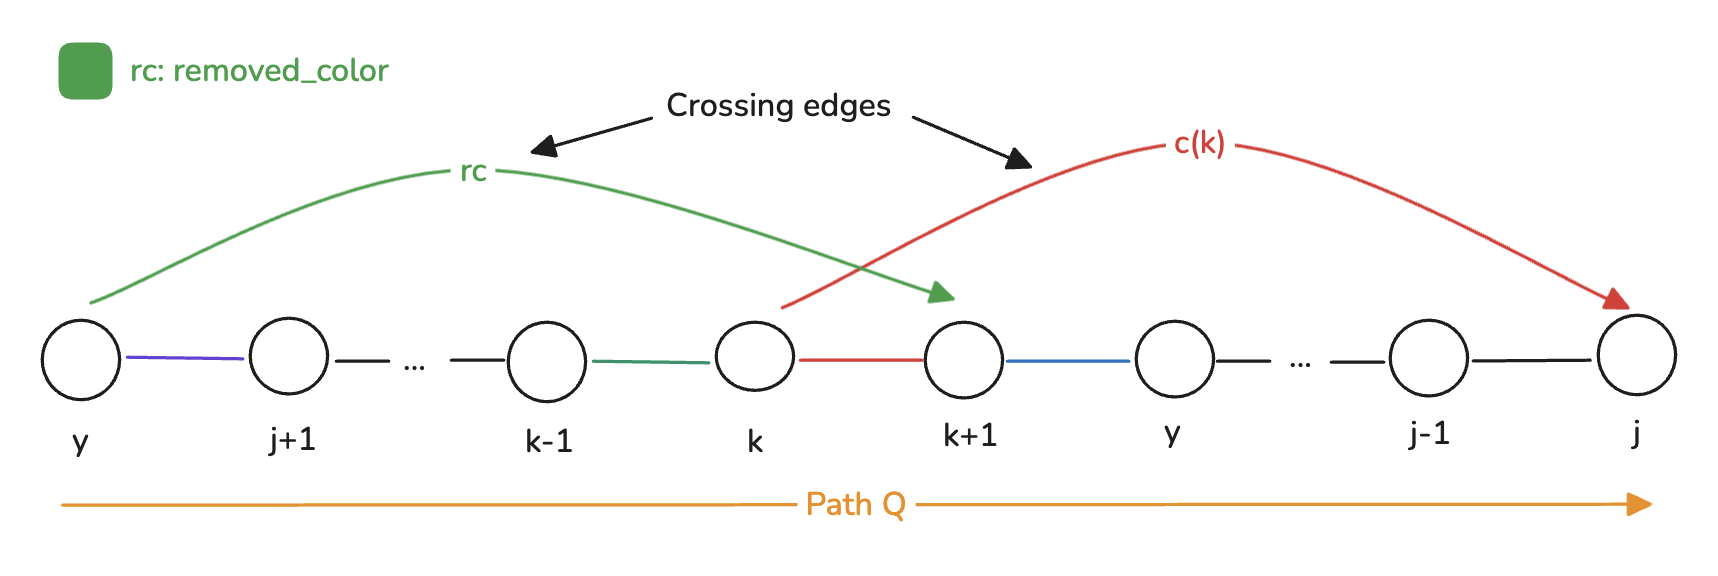
\includegraphics[width=1\textwidth]{figuras/cycle_n-1_last_crossing.png}
    \caption{Final crossing for the case $d^-_D(y) < \frac{n}{2}$ and $P\_vertices[k] \neq y$.}
    \label{fig:cycle_n-1_last_crossing}
\end{figure}

The algorithm to find the answer in this case is the following:

\begin{algorithm}[H]
    \caption{Part 8: Cycle Extension for \( \ell < n - 1 \). Case \( d^-_D(y) < \frac{n}{2} \)}
    \begin{algorithmic}[1]
        \Function{Extend\_Cycle}{$G, C$}
            \State $Q \gets None$
            \State $removed\_color \gets -1$

            \For{$j \in [2, \dots, n - 1]$}
                \State $edge \gets G.check\_edge(y, C.vertices[(j + 1) \bmod n], cy)$
                \If{$edge$ is $None$ or $in\_degree[C.vertices[j]] \neq \lfloor \frac{n}{2} - 1 \rfloor$}
                    \State \textbf{continue}
                \EndIf
                \State $Q\_vertices \gets [y] + C.vertices[j + 1:] + C.vertices[:j + 1]$
                \State $Q\_edges \gets [edge] + C.edges[j + 1:] + C.edges[:j]$
                \State $removed\_color \gets C.edges[j].color$
                \State $Q \gets$ \Call{Path}{$G, Q\_vertices, Q\_edges$}
                \State \textbf{break}
            \EndFor

            \If{$Q$ is $None$}
                \State \textbf{raise} RuntimeError("Did not find Path Q :(")
            \EndIf

            \State $edge \gets check\_edge(G, Q.vertices[-1], Q.vertices[0], removed\_color)$
            \If{$edge$ is not $None$}
                \State \Return \Call{Cycle}{$G, Q.vertices, Q.edges + [edge]$}
            \EndIf

            \State $J0 \gets []$
            \For{$i \in [0, \dots, n - 2]$}
                \State $edge \gets G.check\_edge(Q.vertices[0], Q.vertices[i + 1], removed\_color)$
                \If{$edge$ is not $None$}
                    \State $J0.append((i, edge))$
                \EndIf
            \EndFor

            \State $position \gets [0] \times n$
            \For{$i \in [0, \dots, n - 1]$}
                \State $position[Q.vertices[i]] \gets i$
            \EndFor

            \State $inJn \gets [False] \times n$
            \For{$i \in [0, \dots, n - 1]$}
                \State $inJn[position[i]] \gets True$
            \EndFor

            \For{$k, edge\_from\_first \in J0$}
                \If{$not inJn[k]$}
                    \State \textbf{continue}
                \EndIf
                \State $edge\_from\_last \gets get\_edge(G, Q.vertices[n - 1], Q.vertices[k], Q.edges[k].color)$
                \State $new\_vertices \gets Q.vertices[:k+1] + Q.vertices[k+1:][::-1]$
                \State $new\_edges \gets Q.edges[:k] + [edge\_from\_last] + Q.edges[k+1:][::-1] + [edge\_from\_first]$
                \State \Return \Call{Cycle}{$G, new\_vertices, new\_edges$}
            \EndFor

            \State \textbf{raise} Should never reach this point!
        \EndFunction
    \end{algorithmic}
\end{algorithm}
        

\section{Time completity analysis}

We have run the algorithm for different values of $n$ to see how the time complexity behaves.
The results are shown in the figure below:

\begin{figure}[H]
    \centering
    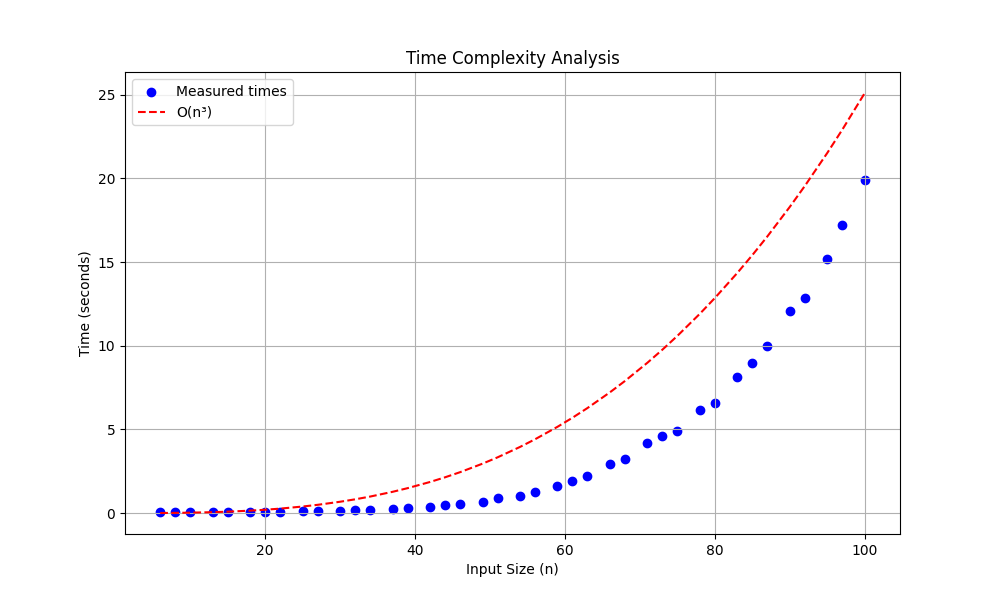
\includegraphics[width=1\textwidth]{figuras/time_complexity.png}
    \caption{Time complexity for different values of $n$.}
    \label{fig:time_complexity}
\end{figure}
